\section{Experiments}

\begin{frame}{1. Paper experiment}
    \textbf{a. Experimental setup}

    \textbf{b. Results}

    \textbf{c. Analysis}
\end{frame}

\begin{frame}{a. Experimental setup}
    
\end{frame}


\begin{frame}{b. Results}

\end{frame}


\begin{frame}{c. Analysis}

\end{frame}


\begin{frame}{2. Re-experiment and Improvements}
\textbf{Pipeline Overview}
\begin{enumerate}
    \item Data Collection
    \item Data Preprocessing
    \item Modeling (Model and Training)
    \item Evaluation \& Comparison
    \item Analysis
\end{enumerate}

\begin{center}
\resizebox{\linewidth}{!}{
\begin{tikzpicture}[
    >=latex,
    node distance=0.8cm and 0.5cm,
    box/.style={draw, rectangle, rounded corners, thick, align=center, fill=blue!10, minimum height=1.2cm, minimum width=3cm},
    proc/.style={draw, rectangle, rounded corners, thick, align=center, fill=yellow!20, minimum height=1.2cm, minimum width=3cm},
    arrow/.style={->, thick}
]

% Nodes
\node[box, fill=green!10] (data) {Data Collection};
\node[proc, right=of data] (pre) {Data Preprocessing};
\node[box, right=of pre, fill=orange!20] (model) {Modeling \\ \small (Model + Training)};
\node[proc, right=of model] (eval) {Evaluation \\ \& Comparison};
\node[box, right=of eval, fill=purple!10] (analysis) {Analysis};

% Arrows
\draw[arrow] (data.east) -- (pre.west);
\draw[arrow] (pre.east) -- (model.west);
\draw[arrow] (model.east) -- (eval.west);
\draw[arrow] (eval.east) -- (analysis.west);

\end{tikzpicture}
}
\end{center}


\end{frame}


%======================
\begin{frame}{a. Datasets \& Data Collection}

Dataset Summary
\begin{center}
\scriptsize
\begin{tabular}{|l|c|c|c|c|c|}
\hline
\textbf{Dataset} & \textbf{Type} & \textbf{\#Samples} & \textbf{\#Subjects} & \textbf{Real / Spoof} & \textbf{Attacks} \\
\hline
CASIA-FASD & Video & 600 & 50 & 150 / 450 & Warp, Cut, Replay \\
\hline
MSU-MFSD & Video & 280 & 35 & 70 / 210 & Print, Replay \\
\hline
NUAA & Image & 12,614 & 15 & 5105 / 7509 & Print \\
\hline
\end{tabular}
\end{center}

\vspace{0.2cm}

\begin{itemize}
    \item \textbf{Sources:} 
\href{http://www.cbsr.ia.ac.cn/english/FaceAntiSpoofDatabases.asp}{CASIA (ICB 2012)}, 
\href{http://biometrics.cse.msu.edu/pubs/databases.html}{MSU (IEEE TIFS 2015)}, 
\href{http://parnec.nuaa.edu.cn/xtan/data/nuaaa.html}{NUAA (ECCV 2010)}
    \item \textbf{Data Types:} Video + Image (Real vs Spoof)
    \item \textbf{Distribution:} Highly imbalanced (spoof $\gg$ real)
\end{itemize}

\end{frame}

%======================

\begin{frame}{a. Datasets \& Data Collection}
\centering

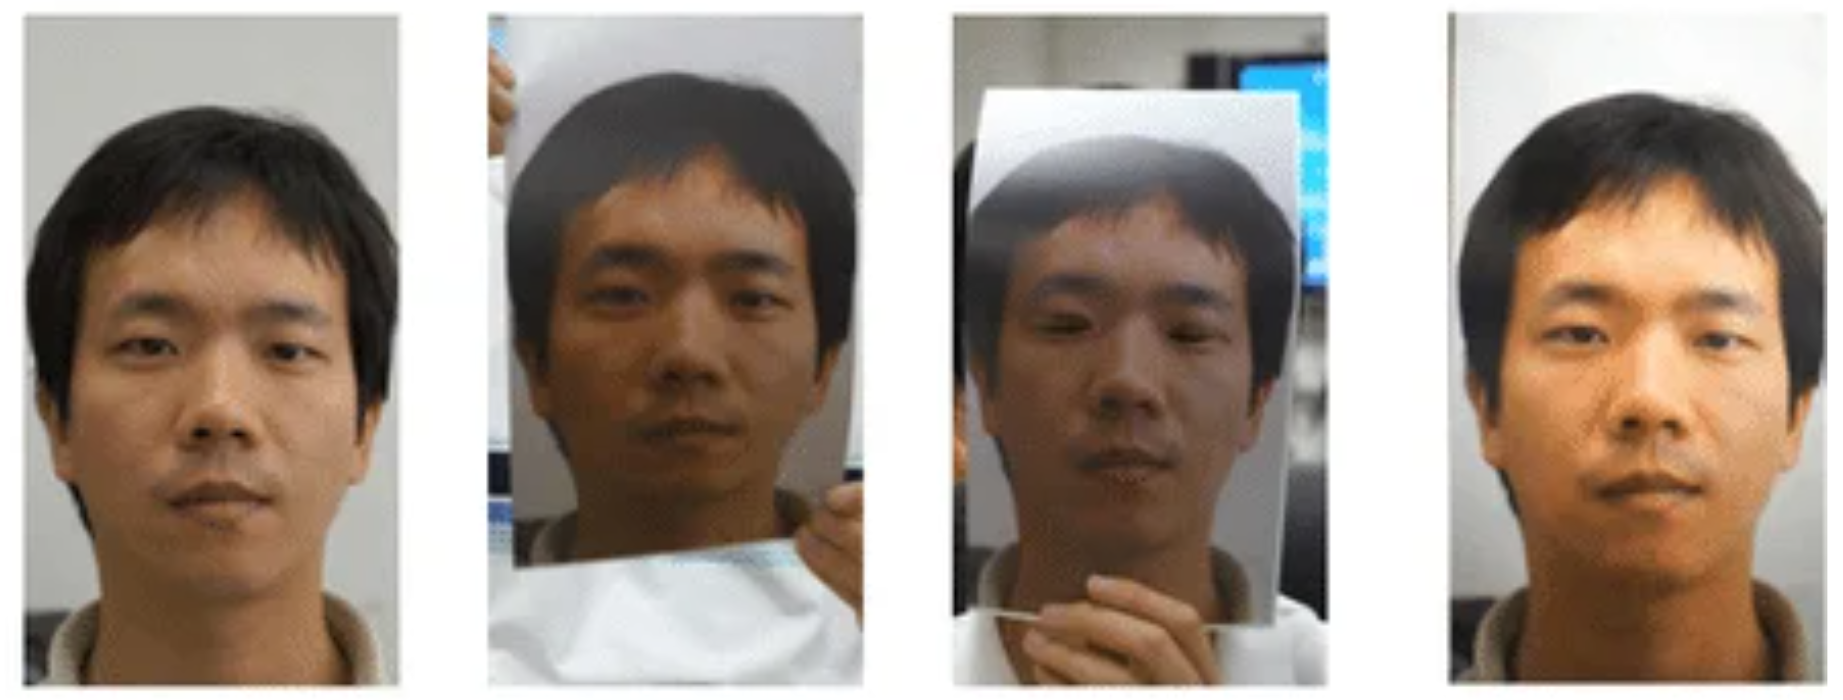
\includegraphics[width=0.4\linewidth,height=2.5cm,keepaspectratio]{img/casia_example.png}
\par\scriptsize CASIA examples

\vspace{0.3cm}

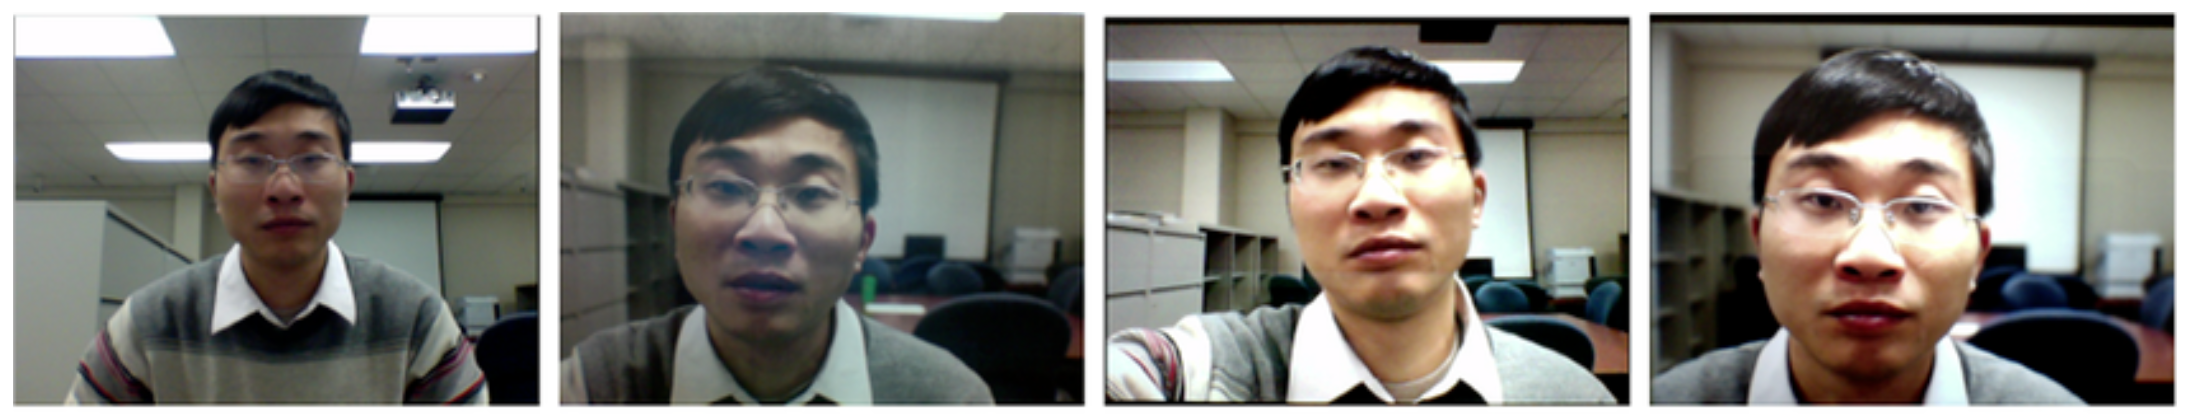
\includegraphics[width=0.6\linewidth,height=2.5cm,keepaspectratio]{img/msu_example.png}
\par\scriptsize MSU-MFSD examples

\vspace{0.3cm}

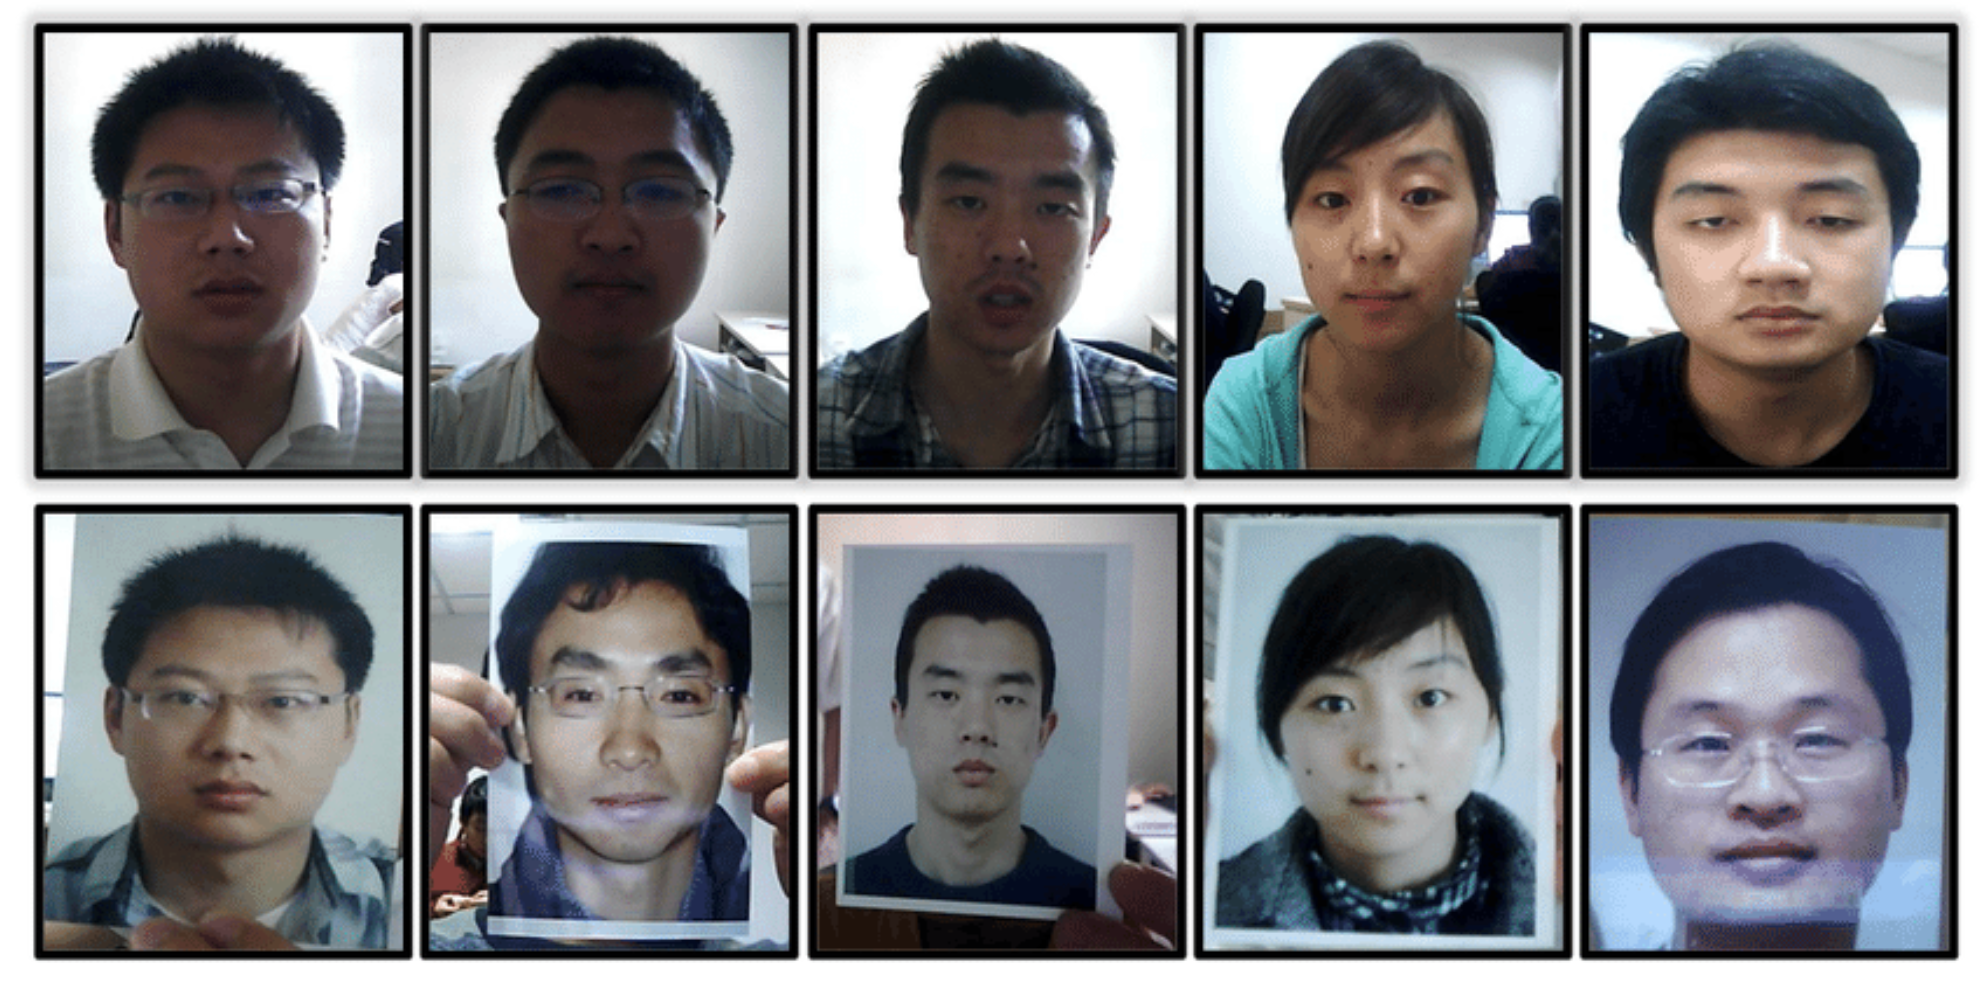
\includegraphics[width=0.8\linewidth,height=2.5cm,keepaspectratio]{img/nuaa_example.png}
\par\scriptsize NUAA examples

\end{frame}


%======================
\begin{frame}{b. Data Preprocessing}

Preprocessing pipeline:
\begin{enumerate}
    \item Face detection (MTCNN)
    \item Depth map generation (PRNet)
    \item Normalization, resizing
    \item Data augmentation
\end{enumerate}


\end{frame}

%======================
\begin{frame}{b. Data Preprocessing}

\textbf{Face detection (MTCNN)}

\vspace{0.3cm}

\textbf{Input:} An RGB image of varying sizes.

\textbf{Output:} Bounding box coordinates, classification confidence scores, and 5 facial landmark coordinates (left eye, right eye, nose, left mouth corner, right mouth corner) for each detected face.


\end{frame}

%======================
\begin{frame}{b. Data Preprocessing}

\begin{figure}[h]
    \centering
    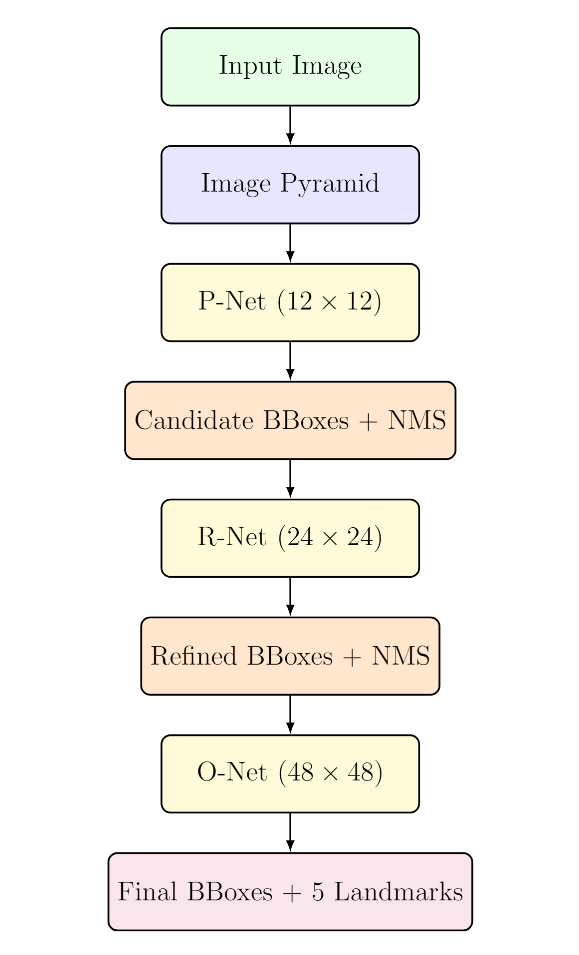
\includegraphics[width=0.37\textwidth]{img/mtcnn.png}
    \caption{MTCNN Architecture}
    \label{fig:example_image}
    
\end{figure}

\end{frame}





%======================
\begin{frame}{b. Data Preprocessing}
\textbf{Depth map generation (PRNet)}

\begin{itemize}
    \item \textbf{Input:} A cropped 2D RGB face image of size $256 \times 256 \times 3$.

    \item \textbf{Output:} A 3D UV Position Map of size $256 \times 256 \times 3$. The channel $Z$ represents the dense 2D depth map of the face.
\end{itemize}



\textbf{Architecture}
\begin{center}
\resizebox{\linewidth}{!}{
\begin{tikzpicture}[
    >=latex,
    node distance=0.5cm and 1cm,
    box/.style={draw, rectangle, rounded corners, thick, align=center, fill=blue!10, minimum height=1.2cm, minimum width=2.5cm},
    augbox/.style={draw, rectangle, rounded corners, thick, align=center, fill=yellow!20, minimum height=1.2cm, minimum width=2.5cm},
    arrow/.style={->, thick}
]

% Nodes
\node[box, fill=green!10] (input) {Cropped RGB \\ \small ($256 \times 256 \times 3$)};
\node[augbox, right=of input] (encoder) {Encoder \\ \small (ResNet-50)};
\node[box, right=of encoder, fill=orange!20] (latent) {Latent Feature \\ \small ($8 \times 8 \times 512$)};
\node[augbox, right=of latent] (decoder) {Decoder \\ \small (ConvTranspose)};
\node[box, fill=purple!10, right=of decoder] (output) {UV Position Map \\ \small ($256 \times 256 \times 3$)};

% Arrows
\draw[arrow] (input.east) -- (encoder.west);
\draw[arrow] (encoder.east) -- (latent.west);
\draw[arrow] (latent.east) -- (decoder.west);
\draw[arrow] (decoder.east) -- (output.west);

\end{tikzpicture}
}
\end{center}

\end{frame}


%======================
\begin{frame}{Implementation}
\begin{itemize}
    \item Code structure overview
    \item Training notebook
    \item Key modules integration
\end{itemize}
\end{frame}

%======================
\begin{frame}{c. Model / Method}
\textbf{Components}
\begin{itemize}
    \item Conv Block
    \item Basic Block
    \item Feature Extractor
    \item Feature Embedder
    \item Depth Estimator
\end{itemize}
\end{frame}




\begin{frame}{c. Model / Method}
\textbf{Conv Block}
\begin{center}
\resizebox{\linewidth}{!}{
\begin{tikzpicture}[
    >=latex, node distance=1cm,
    box/.style={draw, rectangle, rounded corners, thick, align=center, fill=blue!10, minimum width=2.5cm},
    arrow/.style={->, thick}
]

\node[box] (input) {Input};
\node[box, right=of input] (conv) {Conv \\ \small $3\times3$};
\node[box, right=of conv] (norm) {BN / IN \\ \small (AdapNorm)};
\node[box, right=of norm] (relu) {ReLU};
\node[box, right=of relu] (output) {Output};

\draw[arrow] (input) -- (conv);
\draw[arrow] (conv) -- (norm);
\draw[arrow] (norm) -- (relu);
\draw[arrow] (relu) -- (output);

\end{tikzpicture}
}
\end{center}


\textbf{Basic Block}
\begin{center}
\resizebox{\linewidth}{!}{
\begin{tikzpicture}[
    >=latex, node distance=1cm,
    box/.style={draw, rectangle, rounded corners, thick, align=center, fill=blue!10},
    arrow/.style={->, thick}
]

\node[box] (input) {Input};
\node[box, right=of input] (c1) {Conv Block \\ \small $C \to 128$};
\node[box, right=of c1] (c2) {Conv Block \\ \small $128 \to 196$};
\node[box, right=of c2] (c3) {Conv Block \\ \small $196 \to C'$};
\node[box, right=of c3, fill=orange!20] (pool) {MaxPool \\ \small $\downarrow 2$};
\node[box, right=of pool] (output) {Output};

\draw[arrow] (input) -- (c1);
\draw[arrow] (c1) -- (c2);
\draw[arrow] (c2) -- (c3);
\draw[arrow] (c3) -- (pool);
\draw[arrow] (pool) -- (output);

\end{tikzpicture}
}
\end{center}



\end{frame}


\begin{frame}{c. Model / Method}

\textbf{Feature Extractor}
\begin{center}
\resizebox{\linewidth}{!}{
\begin{tikzpicture}[
    >=latex, node distance=0.5cm,
    box/.style={draw, rectangle, rounded corners, thick, align=center, fill=blue!10},
    arrow/.style={->, thick}
]

\node[box] (input) {Input \\ \small 6ch};
\node[box, right=of input] (inc) {Conv Block \\ \small $64$};
\node[box, right=of inc] (d1) {Basic Block \\ \small $128$};
\node[box, right=of d1] (d2) {Basic Block \\ \small $128$};
\node[box, right=of d2] (d3) {Basic Block \\ \small $128$};

\node[box, below=of d2, fill=orange!20] (pool) {Adaptive Pool \\ \small $32\times32$};

\node[box, right=of d3, fill=purple!10] (concat) {Concat \\ \small $dx2, dx3, dx4$};

\draw[arrow] (input) -- (inc);
\draw[arrow] (inc) -- (d1);
\draw[arrow] (d1) -- (d2);
\draw[arrow] (d2) -- (d3);

\draw[arrow] (d2) -- (pool);
\draw[arrow] (d3) -- (concat);
\draw[arrow] (pool) -- (concat);

\end{tikzpicture}
}
\end{center}



\textbf{Feature Embedder}
\begin{center}
\resizebox{\linewidth}{!}{
\begin{tikzpicture}[
    >=latex, node distance=0.5cm,
    box/.style={draw, rectangle, rounded corners, thick, align=center, fill=blue!10},
    arrow/.style={->, thick}
]

\node[box] (input) {Input \\ \small 384ch};
\node[box, right=of input] (c1) {Conv Block \\ \small $128$};
\node[box, right=of c1] (p1) {MaxPool};
\node[box, right=of p1] (c2) {Conv Block \\ \small $256$};
\node[box, right=of c2] (p2) {MaxPool};
\node[box, right=of p2] (c3) {Conv Block \\ \small $512$};
\node[box, right=of c3, fill=orange!20] (gap) {Global Avg Pool};
\node[box, right=of gap, fill=purple!10] (fc) {FC \\ \small 2-dim};

\draw[arrow] (input) -- (c1);
\draw[arrow] (c1) -- (p1);
\draw[arrow] (p1) -- (c2);
\draw[arrow] (c2) -- (p2);
\draw[arrow] (p2) -- (c3);
\draw[arrow] (c3) -- (gap);
\draw[arrow] (gap) -- (fc);

\end{tikzpicture}
}
\end{center}


\textbf{Depth Estimator}
\begin{center}
\resizebox{\linewidth}{!}{
\begin{tikzpicture}[
    >=latex, node distance=1cm,
    box/.style={draw, rectangle, rounded corners, thick, align=center, fill=blue!10},
    arrow/.style={->, thick}
]

\node[box] (input) {Input \\ \small 384ch};
\node[box, right=of input] (c1) {Conv Block \\ \small $128$};
\node[box, right=of c1] (c2) {Conv Block \\ \small $64$};
\node[box, right=of c2] (c3) {Conv Block \\ \small $1$};
\node[box, right=of c3, fill=purple!10] (output) {Depth Map};

\draw[arrow] (input) -- (c1);
\draw[arrow] (c1) -- (c2);
\draw[arrow] (c2) -- (c3);
\draw[arrow] (c3) -- (output);

\end{tikzpicture}
}
\end{center}





\end{frame}





%======================
\begin{frame}{Improvements}
\begin{itemize}
    \item Backbone switching
    \item Data augmentation strategies
    \item Training optimization
\end{itemize}
\end{frame}

%======================
\begin{frame}{d. Training Setup}
\begin{itemize}
    \item Hardware configuration
    \item Loss functions (3 losses)
    \item Optimizer: Adam
    \item Hyperparameters:
    \begin{itemize}
        \item Batch size
        \item Learning rate
        \item Epochs
    \end{itemize}
\end{itemize}
\end{frame}

%======================
\begin{frame}{e. Evaluation Metrics}
\begin{itemize}
    \item Accuracy
    \item AUC
    \item HTER
\end{itemize}
\end{frame}

%======================
\begin{frame}{f. Experiment Setup}
\begin{itemize}
    \item Folder organization
    \item Training pipeline workflow
    \item Seed fixing
    \item Train / Test split
    \item Logging system
    \item Model checkpoint saving
    \item Visualization
\end{itemize}
\end{frame}

%======================
\begin{frame}{Experiment Control}
\begin{itemize}
    \item Reproducibility
    \item Seed fixing
    \item Controlled experiments
\end{itemize}
\end{frame}

%======================
\begin{frame}{g. Results \& Analysis}
\begin{itemize}
    \item Training Analysis
    \item Performance tables
    \item Comparison with baselines
\end{itemize}
\end{frame}

%======================
\begin{frame}{Training Analysis}
\begin{itemize}
    \item Training loss curves
    \item Convergence behavior
\end{itemize}
\end{frame}

%======================
\begin{frame}{Visualization}
\begin{itemize}
    \item t-SNE visualization
    \item Feature maps
\end{itemize}
\end{frame}




